% !TeX root = Phase1.tex
% !TeX program = pdflatex
% Standalone submission source. Compile this file to produce Phase1.pdf.
% Bibliography is embedded; no separate BibTeX run is required.
\documentclass[11pt,a4paper]{article}

\usepackage[T1]{fontenc}
\usepackage[utf8]{inputenc}
\usepackage{lmodern}
\usepackage{microtype}
\usepackage[a4paper,margin=2.5cm]{geometry}
\usepackage{setspace}
\usepackage{booktabs}
\usepackage{longtable}
\usepackage{tabularx}
\usepackage{xcolor}
\usepackage{tikz}
\usetikzlibrary{arrows.meta,positioning,shapes.geometric}
\usepackage[section]{placeins}
\usepackage{natbib}
\usepackage[hidelinks]{hyperref}
\usepackage{float}
\usepackage{array}
\usepackage{graphicx}
\usepackage{enumitem}  %
\usepackage[most]{tcolorbox}

\setstretch{1.08}
\setlength{\parindent}{0pt}
\setlength{\parskip}{0.55em}
\renewcommand{\arraystretch}{1.15}
\newcommand{\placeholder}[1]{\textcolor{gray}{[TODO: #1]}}


% BEGIN embedded wordcount.tex
\newcommand{\mainwordcount}{2017}

% END embedded wordcount.tex


\begin{document}

\hypersetup{pageanchor=false}
\begin{titlepage}
\centering
\vspace*{3cm}
{\Large Eindhoven University of Technology\par}
\vspace{1.5cm}
{\huge\bfseries AI-Supported Sustainability Self-Assessment for TU/e Research\par}
\vspace{0.6cm}
{\Large ENSU -- Retained Phase 1 Report\par}
{\Large Group Q\par}
\vfill
\begin{tabularx}{0.95\textwidth}{@{}lX@{}}
Course: & 5ARF0 Ethics of AI: Theory and Practice \\
Clients: & Philip Nickel and Tijn Borghuis \\
Primary coach: & Qin Tao (Tata) Zeng \\
Stage 1 submission: & 18 September 2026 \\
Word count: & \mainwordcount{} (Stage 1 main text)
\end{tabularx}

\vspace{1cm}
\begin{tabularx}{0.95\textwidth}{@{}p{0.30\textwidth}p{0.13\textwidth}X@{}}
\toprule
Name & Student ID & Email \\
\midrule
Yehao Chen & 2216655 & \href{mailto:y.chen13@student.tue.nl}{\nolinkurl{y.chen13@student.tue.nl}} \\
Dennis de Hoon & 1732773 & \href{mailto:d.b.a.d.hoon@student.tue.nl}{\nolinkurl{d.b.a.d.hoon@student.tue.nl}} \\
Gerald Tobenna Eluagu & 2419289 & \href{mailto:g.t.eluagu@student.tue.nl}{\nolinkurl{g.t.eluagu@student.tue.nl}} \\
Peng Wang & 2342944 & \href{mailto:p.wang1@student.tue.nl}{\nolinkurl{p.wang1@student.tue.nl}} \\
\bottomrule
\end{tabularx}

\vspace{0.6cm}
{\footnotesize Main-text count excludes headings, tables, figures, references, appendices and draft placeholders.\par}

\vfill
\end{titlepage}
\hypersetup{pageanchor=true}


% Historical Phase 1 report only. Phase 2 submission is Assignment 2.tex.

% BEGIN embedded chapters/phase1-body.tex
\section{Introduction and Motivation}

\subsection{Topic, Motivation, Values and Needs}
According to TU/e's Sustainability Visioning Report, sustainable development is a major part of campus development, with the aim of fully embedding sustainability and proactively engaging with societal challenges by 2050 \citep{tue_sustainability_2021}. However, researchers need to translate these ambitions into practical activities involving specific equipment and data. This project explores whether AI can help in this process while remaining transparent and supporting human judgement.

In the client Q\&A, Nickel described the existing self-assessment as a basis for reflection and did not envisage an additional research approval procedure (Appendix~\ref{app:process}).

\subsection{Objectives and Key Terms}
In this project, an AI support tool is proposed to help users judge and examine the potential environmental impacts, taking equipment use, runtime, electricity consumption and other relevant factors into account.

A large language model (LLM) is a language model with a large number of parameters, trained on extensive text data to support language understanding and generation. Here, the LLM would provide supported suggestions based on the provided description of activities while a separate module would use formulas to calculate selected environmental impacts.

The design objective is to help researchers reflect on their own projects using reliable information. The proposed workflow comprises plan submission, AI-assisted activity analysis, formula-based impact estimation, comparison with relevant reference cases, and feedback with practical recommendations. The initial design would show separate indicators without an overall score, because weighting different values requires agreement. The database would be based on published data and findings, and would also include reviewed examples. Missing information should trigger questions or qualified feedback. Evaluation would examine evidence traceability, consistency and whether users find the feedback helpful when revising their plans.

\subsection{Context and Scope}

The project focuses on the research domain at TU/e. Its intended users are researchers, including students conducting research, who want to reflect on the environmental impacts of their planned research activities. This tool is designed for planning and revising research activities, such as data processing and computational experiments. The assessment covers selected environmental impacts for which sufficient activity data and reference information are available.
The tool will not be used to manage campus facilities, evaluate university curricula, or decide which projects receive approval or funding. It will not provide a complete life-cycle assessment or rank researchers and projects across disciplines.

\subsection{Tools, Methods and Frameworks}
The proposed system would be guided by two design methodologies:

1) \textbf{The Value Sensitive Design (VSD) framework.} We would use VSD to identify stakeholder values and translate them into design requirements \citep{friedman2019shaping,vsdlab}. Academic integrity would be supported by protecting unpublished ideas and tracing recommendations to their sources. Resource use, including electricity, would also be considered. Conceptual investigation would identify conflicts such as sustainability versus research quality; client and user feedback would inform the empirical investigation. Technical investigation would test the resulting requirements against the prototype. For example, the scoring conflict leads to separate indicators rather than one overall score.

2) \textbf{The iterative engineering design process.} As the software cannot be built perfectly on the first attempt, we would use an iterative cycle: requirements, prototype, expert evaluation and refinement. The local repository could be updated when TU/e policies change, but new references would require approval and version tracking before use. Outputs could be supported through Retrieval-Augmented Generation (RAG) with relevant TU/e documents; retrieval alone would not guarantee accurate advice.

\textbf{As for the tools:}

1) To lay the groundwork, we would consider \textbf{Llama 3 (8B) or Mistral (7B)} for local deployment. These remain candidate models; their resource use and output quality would need testing. Local hosting alone would not ensure privacy.

2) \textbf{The retrieval engine (RAG stack)} would ground the LLM in selected references and TU/e guidance. A vector database, such as Chroma DB or Qdrant, could be used alongside LangChain or LlamaIndex. The choice has not yet been tested.

3) \textbf{Streamlit or Gradio} could be used to create a web dashboard. An expert panel would allow authorised maintainers to review references and upload updated policy files. Researchers would be able to correct activity information; changes to institutional criteria would require review. HTML, CSS and JavaScript may also be explored.

The original architecture and interface sketches are retained in Appendix~\ref{app:mockup}. The current proposal uses separate indicators rather than the early mock-up's overall score.

\clearpage
\section{Initial Results}

\subsection{Preliminary Literature Search}

The preliminary literature review focuses on campus sustainability, LLMs or RAG, and value-sensitive design. The available record contains course readings and targeted source checks; it does not establish a completed Scopus or IEEE Xplore search. A follow-up search in these databases would combine terms such as ``smart university'' or ``campus sustainability'' with ``LLM'' or ``RAG'' using Boolean operators.

Sources would be screened first for title and abstract relevance, followed by full-text evaluation. Recent implementation studies would be considered alongside foundational VSD work. Studies of local systems are relevant to the proposed deployment, but non-AI methods are also needed as a baseline. No screening total is reported because the original search log is unavailable.

Two questions remain open: how much computing resource a locally hosted model would require, and how subject experts could review and update its references. These are questions for the project rather than established gaps across the whole literature.

\begin{table}[htbp]
\centering
\small
\begin{tabularx}{\textwidth}{@{}p{0.16\textwidth}p{0.12\textwidth}XXp{0.18\textwidth}@{}}
\toprule
Source & Type & Main finding & Need or value & Design implication \\
\midrule
\citet{friedman2019shaping}
& Academic book  
& Technology design involves values that need conceptual, empirical and technical investigation.
& Consider privacy alongside environmental resource use. 
& Provide an expert panel with reviewed source updates and clear responsibilities.  \\
\midrule
\citet{friedman2019shaping}
& Academic book
& Stakeholder values should inform the design and evaluation of technology. & Researchers need to retain the final say over their research plans and be able to correct activity information.
& The design would allow researchers to correct inputs and authorised maintainers to review TU/e policy updates \\
\bottomrule
\end{tabularx}
\caption{Selected literature and implications for the design.}
\label{tab:literature}

\end{table}

\FloatBarrier
\subsection{Design Strategy}

Step 1: Our process begins with going through past literature texts on this topic and gathering data from real-world users (client meetings). Through this, we aim to identify the values and needs of TU/e researchers.

Step 2: Once we are done talking to the clients, we will take their main problems and turn it into a list of rules for our tool. Examples are telling it to check the user's input against the TU/e rulebook and give them advice on how to make it greener, or exploring local deployment on TU/e computers alongside access controls to protect research data.

Step 3: We draw a simple visual layout of our system so users can see how it works (Figure~\ref{fig:workflow}).

Step 4: We show the mock-up to experts and use their feedback to revise the design.


\FloatBarrier
\subsection{Initial Requirements and Constraints}

\begin{table}[H]
\centering
\small
\begin{tabularx}{\textwidth}{|c|c|X|X|X|}
\hline
\textbf{ID} & \textbf{Type} & \textbf{Requirement or constraint} & 
\textbf{Rationale or source} & \textbf{How to check it} \\
\hline

R1 & Functional &
The tool needs to allow researchers to describe their work in their own words. &
This is important to make the tool easily usable. &
Test with example research projects. \\
\hline

R2 & Functional &
The tool has to identify selected environmental impacts and show separate indicators, without an overall score. &
This is the main purpose of the tool. &
Provide the tool with examples of research that have different sustainability impacts. \\
\hline

R3 & Constraint &
The tool needs to make clear that it is not an official approval, but a guideline. &
Sustainability is complex and AI alone will not be enough to make a final judgement. &
Check advisory wording, human review and visible data gaps.\\
\hline

R4 & Constraint &
The researcher decides on changes; developers remain responsible for calculation checks and an institutional maintainer for reviewing guidance. &
Users, developers and maintainers have different responsibilities \citep{santoni2018control}. &
Check that the output identifies decision responsibility and a route for correcting errors \\
\hline

R5 & Constraint & Store only necessary case data; require consent and reviewed source updates. & Privacy and archive governance. & Test access controls, consent and source version records. \\
\hline
R6 & Evaluation & Compare the AI-assisted version with a non-AI checklist using the same evidence and formulas. & Additional resource use requires justification \citep{lin2023cost}. & Compare unsupported advice, correction effort and resource use. \\
\hline

\end{tabularx}
\caption{Initial requirements and constraints}
\label{tab:requirements}
\end{table}

Identifying sustainability impacts is the main requirement and the initial goal of the tool. Researchers, including students performing research, will use the tool to find out what parts of their research potentially form a problem for sustainability. 
Environmental, social and economic considerations inform the sustainability discussion; the initial assessment is limited to selected environmental impacts, as specified in Section~1.3. The output of the tool is only a guideline for the user so that they can improve their research. Researchers retain responsibility for research decisions; this does not remove the responsibilities of developers and maintainers.

\newpage
\FloatBarrier
\subsection{Anticipated Function and Purpose of the Tool}
\begin{itemize}
    \item \textbf{User and immediate goal:} TU/e researchers wanting to know the sustainability impact of their research.
    
    \item \textbf{Input:} A precise description of the research.
    
    \item \textbf{System actions:} The tool analyzes the research for potential sustainability impacts and, if needed, asks follow-up questions.
    
    \item \textbf{Output:} A guideline for researchers explaining how their research impacts sustainability.
    
    \item \textbf{Human review or correction:} Researchers need to carefully review the feedback from the tool.
    
    \item \textbf{Handling of missing information or uncertainty:} Missing information prompts follow-up questions; unresolved gaps are reported and unsupported estimates are withheld.
\end{itemize} 

For this scenario, a TU/e researcher describes their work to the tool. Their research is about developing a new battery for electric cars. 
Potential impacts include obtaining and producing the materials required for the battery. Production requires energy and may involve substantial costs. The tool would consider production impacts where suitable data are available.
The tool will ask questions about the materials used for the production of the new battery. With this information, the tool can then ask further questions about energy use and other relevant inputs. 
When sufficient information is available, the tool could provide guidance on potential impacts, with explanations and possible improvements. Unresolved gaps would remain visible. 
It is now up to the researchers to review the guidelines from the tool and decide what they want to change. The output is not official research approval; responsibility for calculation errors and outdated guidance still needs to be assigned, as described in R4.


Figure~\ref{fig:workflow} summarises the proposed workflow; Figure~\ref{fig:activity} applies it to the battery research example. AI would organise descriptions and draft source-supported suggestions, while explicit calculations would be performed by a separate module. Unresolved data gaps would be disclosed and unsupported estimates withheld.

A proposed TU/e sustainability archive would store comparable research cases with activity conditions, model and advice versions, and follow-up evidence under pseudonymous identifiers. For battery research, records could link a change in a fabrication procedure to subsequent material use and electricity measurements. AI could assist with organising records and identifying relevant cases; an authorised campus curator would approve evidence and guidance updates. Researcher-confirmed outcomes would inform later suggestions, subject to consent and comparability checks. The initial version would record separate indicators and outcome evidence, without an overall score. Archive roles and resources remain to be agreed with the client.

Figure~\ref{fig:workflow} places the requirements at the relevant decisions: input confirmation (R1), separate advisory indicators and uncertainty (R2--R3), and optional case sharing with reviewed access (R4--R5). Declining case reuse would not prevent self-assessment. Consent would authorise only the selected archive access, not public disclosure; access protection and source review would remain institutional responsibilities.


% BEGIN embedded figures/proposed-workflows.tex
\begin{figure}[p]
\centering
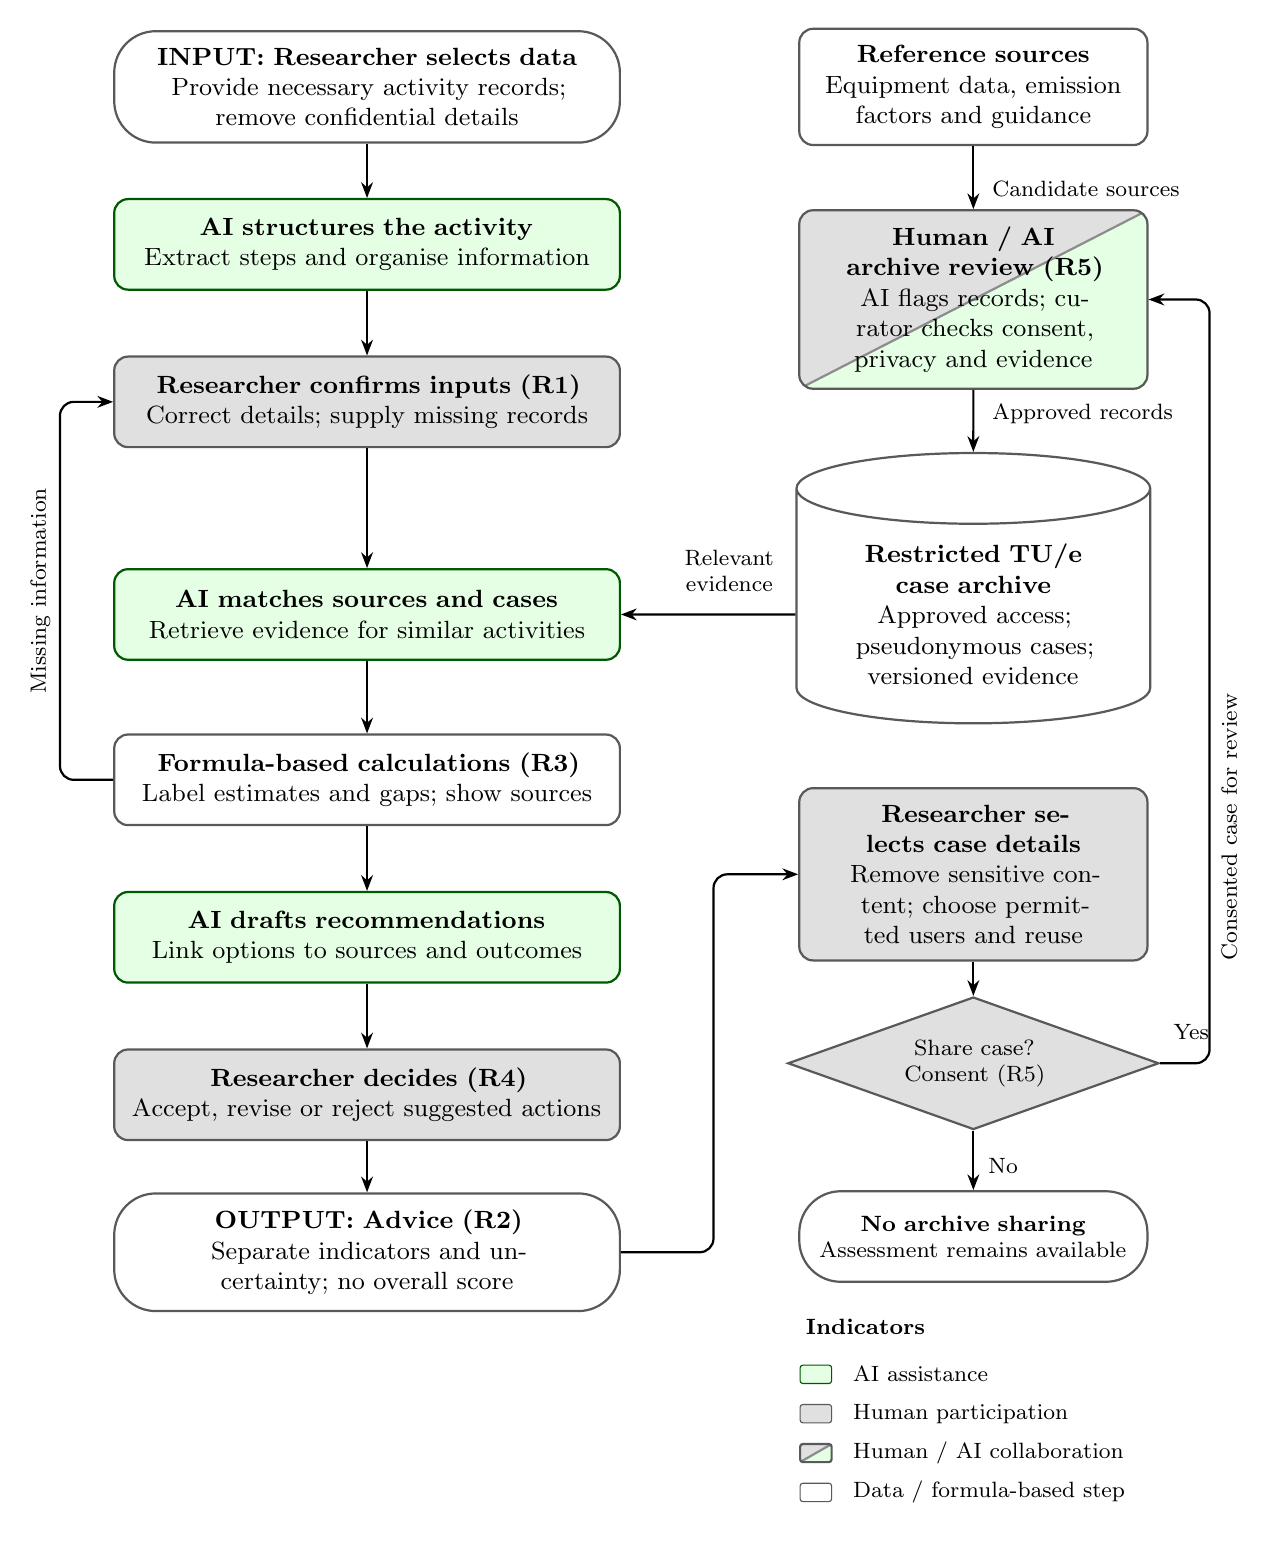
\begin{tikzpicture}[
 base/.style={draw=black!65,thick,rounded corners=5pt,text width=6cm,
 align=center,font=\small,minimum height=1.15cm,inner sep=6pt},
 ai/.style={base,draw=green!35!black,fill=green!10},
 human/.style={base,fill=black!12},
 process/.style={base,fill=white},
 terminal/.style={base,rounded corners=15pt,fill=white},
 side/.style={text width=4cm},
 mixed/.style={base,side,fill=black!12,path picture={
 \fill[green!10] (path picture bounding box.south west)--(path picture bounding box.north east)--(path picture bounding box.south east)--cycle;
 \draw[black!45] (path picture bounding box.south west)--(path picture bounding box.north east);}},
 flow/.style={-{Stealth[length=2mm]},thick,rounded corners=5pt},
 note/.style={font=\footnotesize,align=center,inner sep=1pt}]
\node[terminal] (input) at (0,0) {\textbf{INPUT: Researcher selects data}\\Provide necessary activity records; remove confidential details};
\node[ai] (extract) at (0,-2) {\textbf{AI structures the activity}\\Extract steps and organise information};
\node[human] (check) at (0,-4) {\textbf{Researcher confirms inputs (R1)}\\Correct details; supply missing records};
\node[ai] (match) at (0,-6.7) {\textbf{AI matches sources and cases}\\Retrieve evidence for similar activities};
\node[process] (calc) at (0,-8.8) {\textbf{Formula-based calculations (R3)}\\Label estimates and gaps; show sources};
\node[ai] (draft) at (0,-10.8) {\textbf{AI drafts recommendations}\\Link options to sources and outcomes};
\node[human] (review) at (0,-12.8) {\textbf{Researcher decides (R4)}\\Accept, revise or reject suggested actions};
\node[terminal] (output) at (0,-14.8) {\textbf{OUTPUT: Advice (R2)}\\Separate indicators and uncertainty; no overall score};
\foreach \a/\b in {input/extract,extract/check,check/match,match/calc,calc/draft,draft/review,review/output}
 \draw[flow] (\a)--(\b);
\draw[flow] (calc.west)--(-3.9,-8.8)--(-3.9,-4)--(check.west);
\node[note,rotate=90] at (-4.15,-6.4) {Missing information};

\node[process,side] (refs) at (7.7,0) {\textbf{Reference sources}\\Equipment data, emission factors and guidance};
\node[mixed] (curate) at (7.7,-2.7) {\textbf{Human / AI archive review (R5)}\\AI flags records; curator checks consent, privacy and evidence};
\node[cylinder,shape border rotate=90,aspect=0.2,draw=black!65,thick,
 fill=white,text width=4cm,align=center,font=\small,minimum height=2.35cm,inner sep=7pt]
 (db) at (7.7,-6.7) {\textbf{Restricted TU/e case archive}\\Approved access; pseudonymous cases; versioned evidence};
\node[human,side] (follow) at (7.7,-10.0) {\textbf{Researcher selects case details}\\Remove sensitive content; choose permitted users and reuse};
\node[diamond,aspect=2.8,draw=black!65,thick,fill=black!12,text width=2.5cm,align=center,font=\footnotesize,inner sep=2pt] (consent) at (7.7,-12.4) {Share case?\\Consent (R5)};
\node[terminal,side,font=\footnotesize] (private) at (7.7,-14.6) {\textbf{No archive sharing}\\Assessment remains available};
\draw[flow] (refs)--(curate);
\node[note,anchor=west] at (7.9,-1.3) {Candidate sources};
\draw[flow] (curate)--(db);
\node[note,anchor=west] at (7.9,-4.15) {Approved records};
\draw[flow] (db.west)--(match.east);
\node[note] at (4.6,-6.15) {Relevant\\evidence};
\draw[flow] (output.east)--(4.4,-14.8)--(4.4,-10.0)--(follow.west);
\draw[flow] (follow)--(consent);
\draw[flow] (consent.east)--(10.7,-12.4)--(10.7,-2.7)--(curate.east);
\node[note,anchor=west] at (10.2,-12.0) {Yes};
\draw[flow] (consent)--(private);
\node[note,anchor=west] at (7.85,-13.7) {No};
\node[note,rotate=90] at (10.95,-9.4) {Consented case for review};

\node[anchor=west,font=\footnotesize\bfseries] at (5.45,-15.75) {Indicators};
\node[draw=green!35!black,rounded corners=1pt,fill=green!10,minimum width=0.4cm,minimum height=0.23cm] at (5.7,-16.35) {};
\node[anchor=west,font=\footnotesize] at (6.05,-16.35) {AI assistance};
\node[draw=black!65,rounded corners=1pt,fill=black!12,minimum width=0.4cm,minimum height=0.23cm] at (5.7,-16.85) {};
\node[anchor=west,font=\footnotesize] at (6.05,-16.85) {Human participation};
\node[mixed,text width=0cm,minimum width=0.4cm,minimum height=0.23cm,inner sep=0pt,rounded corners=1pt] at (5.7,-17.35) {};
\node[anchor=west,font=\footnotesize] at (6.05,-17.35) {Human / AI collaboration};
\node[draw=black!65,rounded corners=1pt,fill=white,minimum width=0.4cm,minimum height=0.23cm] at (5.7,-17.85) {};
\node[anchor=west,font=\footnotesize] at (6.05,-17.85) {Data / formula-based step};
\end{tikzpicture}
\caption{Proposed self-assessment workflow with optional case sharing and curator review. Requirement IDs link decisions to Table~\ref{tab:requirements}.}
\label{fig:workflow}
\end{figure}

\begin{figure}[!htbp]
\centering
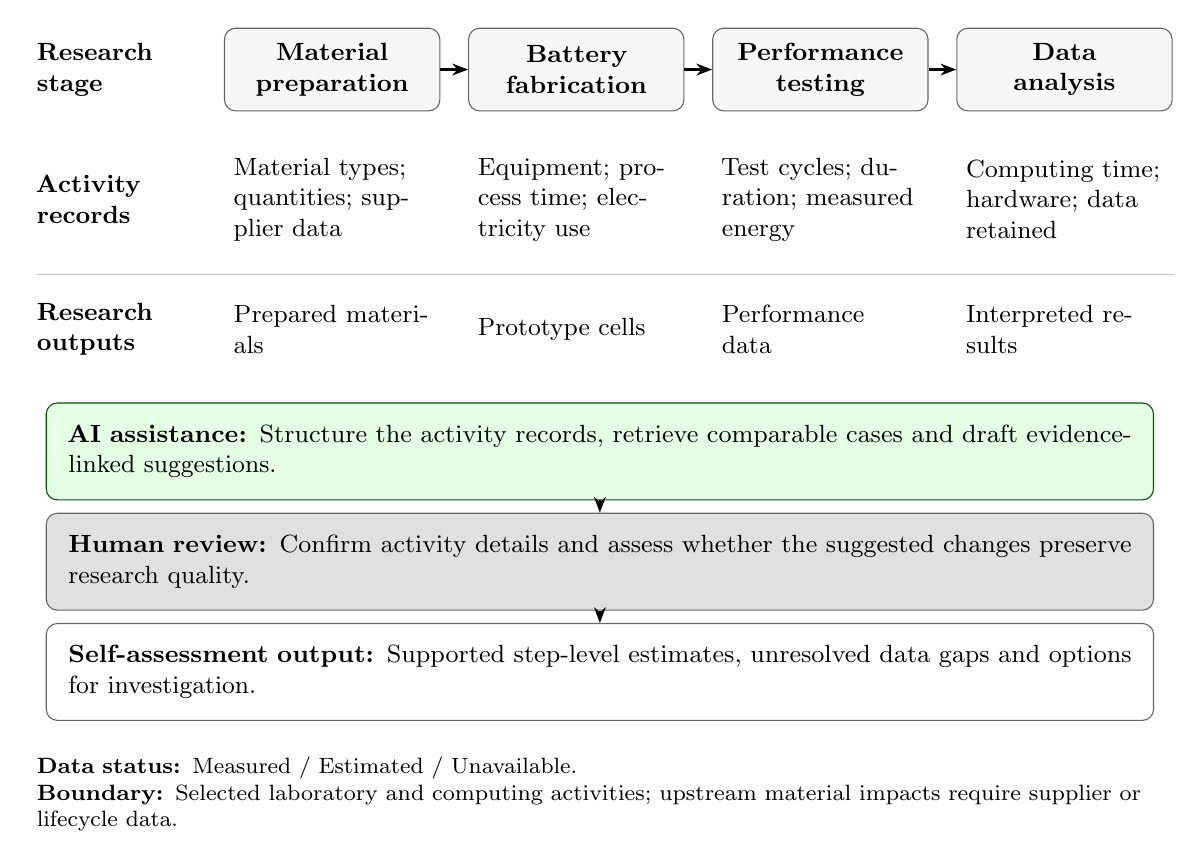
\begin{tikzpicture}[
 stagebox/.style={draw=black!60,rounded corners=4pt,fill=black!3,text width=2.5cm,minimum height=1.05cm,align=center,font=\small\bfseries},
 cell/.style={text width=2.5cm,align=left,font=\small},
 rowlabel/.style={text width=1.9cm,align=left,font=\small\bfseries},
 flow/.style={-{Stealth[length=2mm]},thick,rounded corners=4pt},
 band/.style={draw=black!60,rounded corners=4pt,text width=13.5cm,align=left,font=\small,inner sep=8pt}]
\node[rowlabel] at (0,0) {Research\\stage};
\node[stagebox] (a) at (2.8,0) {Material\\preparation};
\node[stagebox] (b) at (5.9,0) {Battery\\fabrication};
\node[stagebox] (c) at (9,0) {Performance\\testing};
\node[stagebox] (d) at (12.1,0) {Data\\analysis};
\draw[flow] (a)--(b);\draw[flow] (b)--(c);\draw[flow] (c)--(d);
\node[rowlabel] at (0,-1.65) {Activity\\records};
\node[cell] at (2.8,-1.65) {Material types; quantities; supplier data};
\node[cell] at (5.9,-1.65) {Equipment; process time; electricity use};
\node[cell] at (9,-1.65) {Test cycles; duration; measured energy};
\node[cell] at (12.1,-1.65) {Computing time; hardware; data retained};
\draw[black!25] (-0.95,-2.6)--(13.5,-2.6);
\node[rowlabel] at (0,-3.3) {Research\\outputs};
\node[cell] at (2.8,-3.3) {Prepared materials};
\node[cell] at (5.9,-3.3) {Prototype cells};
\node[cell] at (9,-3.3) {Performance data};
\node[cell] at (12.1,-3.3) {Interpreted results};
\node[band,draw=green!35!black,fill=green!10] (assist) at (6.2,-4.85)
{\textbf{AI assistance:} Structure the activity records, retrieve comparable cases and draft evidence-linked suggestions.};
\node[band,fill=black!12] (verify) at (6.2,-6.25)
{\textbf{Human review:} Confirm activity details and assess whether the suggested changes preserve research quality.};
\draw[flow] (assist)--(verify);
\node[band] (result) at (6.2,-7.65)
{\textbf{Self-assessment output:} Supported step-level estimates, unresolved data gaps and options for investigation.};
\draw[flow] (verify)--(result);
\node[align=left,text width=14.3cm,font=\footnotesize] at (6.2,-9.2)
{\textbf{Data status:} Measured / Estimated / Unavailable.\\
\textbf{Boundary:} Selected laboratory and computing activities; upstream material impacts require supplier or lifecycle data.};
\end{tikzpicture}
\caption{Illustrative battery research stages, records and outputs used for self-assessment. Green denotes AI assistance; grey denotes human review.}
\label{fig:activity}
\end{figure}

% END embedded figures/proposed-workflows.tex



\FloatBarrier
\subsection{Projected Users, Stakeholders and Values}
\begin{table}[ht]
\centering
\begin{tabularx}{\textwidth}{|X|X|X|X|}
\hline
\textbf{Stakeholder} & \textbf{Role or relationship to the tool} & 
\textbf{Expected benefit} & \textbf{Concern or burden} \\
\hline

TU/e researchers &
Main users &
Identify impact on sustainability &
Time needed to provide information \\
\hline

Students &
Main users &
Same as researchers &
Possible overreliance on the tool \\
\hline

Supervisors &
Support &
Get a better understanding to help &
Extra time needed to review the output 
\\
\hline

TU/e sustainability team &
Experts &
Potential improvement or addition to the existing tool &
Time needed to understand and review the tool \\
\hline

\end{tabularx}
\caption{Stakeholder notes}
\label{tab:stakeholders}
\end{table}

The TU/e researchers and students will be the main users of our tool. They provide the tool with their research and receive sustainability guidance for their project in return.  Supervisors for the projects performed by the researchers and students will also use this information from the tool but will not need to use the tool directly.  Some stakeholders might have different expectations from the tool, but these are the benefits it is intended to provide.

\FloatBarrier
\clearpage
\section{Discussion}

\subsection{Ethical Issues and Value Conflicts}

The definition of sustainable research determines how activities are assessed. \citet{hasselbalch2025sustainability} locate sustainability within sociotechnical relations of power, making the selection of criteria an ethical issue. If electricity consumption is prioritised, an intensive experiment may be rated unfavourably despite its scientific value. In the proposed assessment, environmental indicators would therefore be presented alongside explanations of research purpose. Comparisons would be restricted to activities with comparable objectives and quality requirements. The initial design therefore omits aggregate scores and cross-disciplinary rankings. Client agreement is still needed on indicator selection and the conditions under which similar activities can be compared.

Numerical estimates may be treated as more authoritative than their evidence warrants. \citet{lacoste2019carbon} identify hardware, runtime and electricity supply as factors affecting emissions from machine learning training. Their method does not establish validity for every research activity. Apparent differences between cases may be smaller than calculation uncertainty. Measured and estimated values would therefore be distinguished, with missing information flagged and sources and boundaries disclosed. Input correction would remain available to researchers. These provisions support scrutiny, but cannot ensure that an assessment is critically examined.

The resource consumption of the assessment tool also requires justification. \citet{lin2023cost} argues for transparency about AI's energy use. Explicit calculations would be assigned to fixed formulas, while AI assistance would support descriptions and suggestions, including retrieval from the reviewed archive. Comparison with a structured non-AI assessment is needed to establish whether any additional benefit warrants the computation and review effort. Environmental improvement has not yet been demonstrated.

\subsection{Design Barriers and Challenges}

Defining a manageable assessment boundary is a practical constraint. Consumption from shared equipment and computing services may be difficult to attribute to individual activities. One representative workflow would be mapped with the client to establish which records are available. Estimates of equipment operation would state their exclusions. Replacement advice would require evidence about manufacturing impacts as well as operating savings.

Reference data and recommendations require maintenance. Sources, review dates and version histories would be recorded so that earlier assessments remain traceable. Following the institutional perspective of \citet{hasselbalch2025sustainability}, responsibility for correcting or withdrawing outdated guidance would need to be assigned at TU/e. The responsible role and available resources remain unresolved. For the proposed campus archive, outcome evidence and comparable activity conditions would require review before cases were reused. Higher assessment scores alone would not demonstrate reduced environmental impact. Reported outcomes would be distinguished from verified measurements, since selective reporting could favour successful cases and bias recommendations for future users of the proposed archive.

Evaluation would compare AI-assisted feedback with a structured checklist on the same cases. Evidence support, omitted issues and correction effort would be examined to establish whether further development is justified.

\begin{table}[!htbp]
\centering
\footnotesize
\setlength{\tabcolsep}{4pt}
\renewcommand{\arraystretch}{1.35}
\begin{tabularx}{\textwidth}{@{}>{\raggedright\arraybackslash}p{0.13\textwidth}>{\raggedright\arraybackslash}p{0.12\textwidth}>{\raggedright\arraybackslash}p{0.14\textwidth}>{\raggedright\arraybackslash}X>{\raggedright\arraybackslash}p{0.20\textwidth}@{}}
\toprule
Risk & Stakeholders & Values & Response and basis & Limitation \\
\midrule
Privacy & Researchers; case contributors & Privacy; autonomy & Minimise stored details; control archive access and case reuse \citep{hasselbalch2025sustainability}. & Activity descriptions may identify a contributor. \\
\midrule
Unclear AI advice & Researchers & Transparency; accountability & Show sources, model version and uncertainty \citep{lacoste2019carbon}. & A retrieved case may be irrelevant or misinterpreted. \\
\midrule
Greenwashing & TU/e; researchers & Sustainability; trust & State boundaries; report separate indicators and observed impacts \citep{lin2023cost}. & Partial indicators need not reflect lower overall impacts. \\
\midrule
Rebound effects & TU/e; affected communities & Environmental impact & Track total activity and resource use alongside efficiency \citep{luccioni2025rebound}. & Savings may encourage additional activity. \\
\midrule
Unfair recommendations & Research groups & Fairness & Compare similar objectives and conditions; review archive coverage \citep{hasselbalch2025sustainability}. & Uneven case contributions can distort comparisons. \\
\midrule
Reduced human control & Researchers; campus curator & Human oversight & Keep decisions with researchers; assign responsibility for archive updates \citep{santoni2018control}. & Formal review does not ensure critical engagement. \\
\bottomrule
\end{tabularx}
\caption{Anticipated ethical risks, literature-informed responses and remaining limitations.}
\label{tab:ethical-risks}
\end{table}

% END embedded chapters/phase1-body.tex

\clearpage
\nocite{*}
\begin{thebibliography}{26}
\providecommand{\natexlab}[1]{#1}
\providecommand{\url}[1]{\texttt{#1}}
\expandafter\ifx\csname urlstyle\endcsname\relax
  \providecommand{\doi}[1]{doi: #1}\else
  \providecommand{\doi}{doi: \begingroup \urlstyle{rm}\Url}\fi

\bibitem[Abrahamse et~al.(2005)Abrahamse, Steg, Vlek, and
  Rothengatter]{abrahamse2005review}
Wokje Abrahamse, Linda Steg, Charles Vlek, and Talib Rothengatter.
\newblock A review of intervention studies aimed at household energy
  conservation.
\newblock \emph{Journal of Environmental Psychology}, 25\penalty0 (3):\penalty0
  273--291, 2005.
\newblock \doi{10.1016/j.jenvp.2005.08.002}.

\bibitem[Berthelot et~al.(2025)Berthelot, Caron, Jay, and
  Lef\`evre]{berthelot2025environmental}
Antoine Berthelot, Eddy Caron, Maxime Jay, and Laurent Lef\`evre.
\newblock Understanding the environmental impact of generative ai services.
\newblock \emph{Communications of the ACM}, 68\penalty0 (7):\penalty0 46--53,
  2025.
\newblock \doi{10.1145/3725984}.

\bibitem[Carver and Scheier(1982)]{carver1982control}
Charles~S. Carver and Michael~F. Scheier.
\newblock Control theory: A useful conceptual framework for personality-social,
  clinical, and health psychology.
\newblock \emph{Psychological Bulletin}, 92\penalty0 (1):\penalty0 111--135,
  1982.
\newblock \doi{10.1037/0033-2909.92.1.111}.

\bibitem[{Eindhoven University of Technology}(2023)]{tue_sustainability_2021}
{Eindhoven University of Technology}.
\newblock Tu/e sustainability visioning report.
\newblock Technical report, TU/e Sustainability Ambassador Office, 2023.
\newblock URL
  \url{https://assets.w3.tue.nl/w/fileadmin/TU_e_Sustainability/Sustainability_Team/Logos/TUe%20Sustainability%20Visioning%20Report%20Spread.pdf}.

\bibitem[{Eindhoven University of Technology}(2025)]{tue_operations_2025}
{Eindhoven University of Technology}.
\newblock Tu/e operations strategy 2026-2030: Curious, open, respectful,
  responsible.
\newblock Technical report, TU/e Managing Directors Council, December 2025.
\newblock URL
  \url{https://assets.w3.tue.nl/w/fileadmin/content/Our_University/About%20our%20university/Publications/TUe%20Operations%20Strategy%202026-2030.pdf}.

\bibitem[{European Commission}(2021)]{eu_ethics_2021}
{European Commission}.
\newblock Ethics by design and ethics of use approaches for artificial
  intelligence.
\newblock Technical report, Directorate-General for Research and Innovation,
  2021.
\newblock URL
  \url{https://ec.europa.eu/info/funding-tenders/opportunities/docs/2021-2027/horizon/guidance/ethics-by-design-and-ethics-of-use-approaches-for-artificial-intelligence_he_en.pdf}.

\bibitem[{European Data Protection Board}(2025)]{edpb2025pseudonymisation}
{European Data Protection Board}.
\newblock Guidelines 01/2025 on pseudonymisation (version for public
  consultation), 2025.
\newblock URL
  \url{https://www.edpb.europa.eu/system/files/2025-01/edpb_guidelines_202501_pseudonymisation_en.pdf}.

\bibitem[{European Parliament and Council of the European
  Union}(2016)]{gdpr2016}
{European Parliament and Council of the European Union}.
\newblock Regulation (eu) 2016/679 (general data protection regulation), 2016.
\newblock URL \url{https://eur-lex.europa.eu/eli/reg/2016/679/oj/eng}.

\bibitem[Friedman and Hendry(2019)]{friedman2019shaping}
Batya Friedman and David~G. Hendry.
\newblock \emph{Value Sensitive Design: Shaping Technology with Moral
  Imagination}.
\newblock MIT Press, 2019.

\bibitem[Friedman et~al.(2003)Friedman, Kahn, and Borning]{friedman2003value}
Batya Friedman, Peter~H. Kahn, Jr., and Alan Borning.
\newblock Value sensitive design and information systems.
\newblock In \emph{Human-Computer Interaction Development Process}, pages
  361--410. CRC Press, 2003.

\bibitem[Hasselbalch and van Wynsberghe(2025)]{hasselbalch2025sustainability}
Gry Hasselbalch and Aimee van Wynsberghe.
\newblock Artificial intelligence, power, and sustainability.
\newblock In Nathalie~A. Smuha, editor, \emph{The Cambridge Handbook of the
  Law, Ethics and Policy of Artificial Intelligence}, pages 117--130. Cambridge
  University Press, 2025.

\bibitem[Hattie and Timperley(2007)]{hattie2007feedback}
John Hattie and Helen Timperley.
\newblock The power of feedback.
\newblock \emph{Review of Educational Research}, 77\penalty0 (1):\penalty0
  81--112, 2007.
\newblock \doi{10.3102/003465430298487}.

\bibitem[Heath et~al.(1999)Heath, Larrick, and Wu]{heath1999goals}
Chip Heath, Richard~P. Larrick, and George Wu.
\newblock Goals as reference points.
\newblock \emph{Cognitive Psychology}, 38\penalty0 (1):\penalty0 79--109, 1999.
\newblock \doi{10.1006/cogp.1998.0708}.

\bibitem[Kahneman and Tversky(1979)]{kahneman1979prospect}
Daniel Kahneman and Amos Tversky.
\newblock Prospect theory: An analysis of decision under risk.
\newblock \emph{Econometrica}, 47\penalty0 (2):\penalty0 263--291, 1979.
\newblock \doi{10.2307/1914185}.

\bibitem[Lacoste et~al.(2019)Lacoste, Luccioni, Schmidt, and
  Dandres]{lacoste2019carbon}
Alexandre Lacoste, Alexandra Luccioni, Victor Schmidt, and Thomas Dandres.
\newblock Quantifying the carbon emissions of machine learning.
\newblock arXiv preprint arXiv:1910.09700, 2019.

\bibitem[Li et~al.(2010)Li, Dey, and Forlizzi]{li2010stages}
Ian Li, Anind Dey, and Jodi Forlizzi.
\newblock A stage-based model of personal informatics systems.
\newblock In \emph{Proceedings of the SIGCHI Conference on Human Factors in
  Computing Systems}, pages 557--566. ACM, 2010.
\newblock \doi{10.1145/1753326.1753409}.

\bibitem[Lin(2023)]{lin2023cost}
Patrick~K. Lin.
\newblock The cost of training a machine: Lighting the way for a climate-aware
  policy framework that addresses artificial intelligence's carbon footprint
  problem.
\newblock \emph{Fordham Environmental Law Review}, 34\penalty0 (2), 2023.
\newblock URL \url{https://ir.lawnet.fordham.edu/elr/vol34/iss2/1/}.

\bibitem[Luccioni et~al.(2025)Luccioni, Strubell, and
  Crawford]{luccioni2025rebound}
Alexandra~Sasha Luccioni, Emma Strubell, and Kate Crawford.
\newblock From efficiency gains to rebound effects: The problem of jevons'
  paradox in {AI}'s polarized environmental debate.
\newblock In \emph{Proceedings of the 2025 ACM Conference on Fairness,
  Accountability, and Transparency}, 2025.
\newblock \doi{10.1145/3715275.3732007}.

\bibitem[Nissenbaum(2004)]{nissenbaum2004privacy}
Helen Nissenbaum.
\newblock Privacy as contextual integrity.
\newblock \emph{Washington Law Review}, 79\penalty0 (1):\penalty0 119--157,
  2004.
\newblock URL \url{https://digitalcommons.law.uw.edu/wlr/vol79/iss1/10/}.

\bibitem[{OECD} and {European Commission Joint Research
  Centre}(2008)]{oecd2008composite}
{OECD} and {European Commission Joint Research Centre}.
\newblock \emph{Handbook on Constructing Composite Indicators: Methodology and
  User Guide}.
\newblock OECD Publishing, Paris, 2008.
\newblock \doi{10.1787/9789264043466-en}.

\bibitem[Santoni~de Sio and van~den Hoven(2018)]{santoni2018control}
Filippo Santoni~de Sio and Jeroen van~den Hoven.
\newblock Meaningful human control over autonomous systems: A philosophical
  account.
\newblock \emph{Frontiers in Robotics and AI}, 5:\penalty0 15, 2018.
\newblock \doi{10.3389/frobt.2018.00015}.

\bibitem[Schultz et~al.(2007)Schultz, Nolan, Cialdini, Goldstein, and
  Griskevicius]{schultz2007norms}
P.~Wesley Schultz, Jessica~M. Nolan, Robert~B. Cialdini, Noah~J. Goldstein, and
  Vladas Griskevicius.
\newblock The constructive, destructive, and reconstructive power of social
  norms.
\newblock \emph{Psychological Science}, 18\penalty0 (5):\penalty0 429--434,
  2007.
\newblock \doi{10.1111/j.1467-9280.2007.01917.x}.

\bibitem[Shiekh and Zhu(2026)]{shiekh2026graduate}
Kylee Shiekh and Qin Zhu.
\newblock Exploring how graduate engineering researchers approach {AI}
  sustainability: Perceptions, design considerations, and impact assessment.
\newblock \emph{International Journal of Technology and Design Education},
  2026.
\newblock \doi{10.1007/s10798-026-10100-y}.
\newblock URL
  \url{https://link.springer.com/article/10.1007/s10798-026-10100-y}.

\bibitem[Shute(2008)]{shute2008feedback}
Valerie~J. Shute.
\newblock Focus on formative feedback.
\newblock \emph{Review of Educational Research}, 78\penalty0 (1):\penalty0
  153--189, 2008.
\newblock \doi{10.3102/0034654307313795}.

\bibitem[{Value Sensitive Design Lab}(n.d.)]{vsdlab}
{Value Sensitive Design Lab}.
\newblock About vsd.
\newblock University of Washington, n.d.
\newblock URL \url{https://vsdesign.org/vsd/}.
\newblock Accessed 18 September 2026.

\bibitem[Zimmerman(2002)]{zimmerman2002self}
Barry~J. Zimmerman.
\newblock Becoming a self-regulated learner: An overview.
\newblock \emph{Theory Into Practice}, 41\penalty0 (2):\penalty0 64--70, 2002.
\newblock \doi{10.1207/s15430421tip4102_2}.

\end{thebibliography}

\appendix
\clearpage

% BEGIN embedded appendices/phase1-process.tex
\section{Documentation of Process}
\label{app:process}
The record below distinguishes available evidence from proposed work. The client Q\&A is documented by an automatic transcript stored with the project; its recording date is not identified in the transcript. Statements are paraphrased and attributed using its timestamps. They provide design context rather than a representative user study.

\begin{longtable}{@{}p{0.17\textwidth}p{0.35\textwidth}p{0.38\textwidth}@{}}
\toprule
Record & Evidence or activity & Implication or output \\
\midrule\endfirsthead
\toprule Record & Evidence or activity & Implication or output \\
\midrule\endhead
Client Q\&A, 0:03--0:28 & Borghuis describes increased household electricity use after installing research computing equipment. & Resource use motivates activity-level assessment; this anecdote is not a measured benchmark. \\
\midrule
Client Q\&A, 1:16--1:55 & Nickel reports completing the existing self-assessment for a research project. & Start from researcher reflection and investigate fit with existing practice. \\
\midrule
Client Q\&A, 6:23--7:19 & Nickel distinguishes reflection and impact communication from an additional institutional go/no-go procedure. & Advisory output; no research approval or unvalidated overall score. \\
\midrule
10 Sep 2026, coaching meeting & Discussion of accountability, transparency, privacy and VSD, with questions about intended users and deployment. & Clarified the issues to address in the design and requirements. \\
\midrule
14 Sep 2026, Teams group meeting & Discussed task allocation, the system concept and the proposed product; coordinated the project timeline. & Agreed the division of work and a shared direction for the product and schedule. \\
\midrule
18 Sep 2026 & Draft consolidation, source checking and diagram revision. & Requirements linked to the baseline, uncertainty handling and archive governance; final group review remains pending. \\
\bottomrule
\caption{Available process evidence and its use in the design.}\\
\end{longtable}

\subsection*{Literature-review record}
The available record documents a targeted review; database screening totals cannot be established from it. On 18 September, source checks used the phrases ``value sensitive design 2019'' (MIT Press), ``value sensitive design conceptual empirical technical'' (VSD Lab), and the exact titles or DOI links of the environmental and human-control references. Course materials supplied the initial sustainability references. A database search with reproducible strings, dates and exclusion reasons remains a next-stage task.

% END embedded appendices/phase1-process.tex

\clearpage

% BEGIN embedded appendices/phase1-planning.tex
\section{Project Planning}
The schedule combines course deadlines with proposed group meetings. Meeting dates are planning targets, not records of completed meetings. Responsibilities below concern the whole group unless an individual obligation is specified; the first meeting would allocate named leads and record each decision.

{\small
\begin{longtable}{@{}p{0.16\textwidth}p{0.45\textwidth}p{0.30\textwidth}@{}}
\toprule Date & Activity and discussion agenda & Output or decision \\
\midrule\endfirsthead
\toprule Date & Activity and discussion agenda & Output or decision \\
\midrule\endhead
18 Sep & Final group review: reconcile sections, check citations and figures, confirm disclosure and allocate submission checks. & Agreed Phase 1 draft; submit by 23:59. \\
\midrule
21 Sep & Group meeting: choose one battery-research activity; agree boundaries, data needs and named task leads. & Case specification and task allocation. \\
\midrule
22--29 Sep & Scheduled coaching: discuss the checklist baseline, advisory scope and potential archive maintainer. & Recorded feedback and questions requiring follow-up. \\
\midrule
25 Sep & Group working session: review reference sources and matching conditions; compare missing-data examples. & Initial source register and checklist. \\
\midrule
30 Sep & Prototype review: check whether each requirement has a visible feature and a test; discuss researcher and curator roles. & Annotated mock-up and requirement updates. \\
\midrule
5 Oct & Group evaluation session, subject to reviewer availability: compare checklist and assisted feedback on identical cases. & Error, correction-effort and resource-use record; unresolved tests logged. \\
\midrule
8--10 Oct & Review evaluation limitations and coaching feedback; agree revisions and prepare practice pitch. & Revised design and Phase 2 draft. \\
\midrule
11 Oct & Submit Phase 2 draft for peer review by 23:59. & Submitted draft. \\
\midrule
14--16 Oct & Discuss received feedback; each member completes individual peer review by 16 Oct, 23:59. & Revision priorities and individual reviews. \\
\midrule
19--20 Oct & Group rehearsal and recording: check that the pitch matches the report and qualifies untested claims. & Video pitch submitted by 20 Oct, 23:59. \\
\midrule
22--23 Oct & Final group check of references, responsibility allocation and remaining limitations. & Phase 2 final report by 23 Oct, 23:59. \\
\midrule
24 Oct & Each member completes the groupmate evaluation. & Individual evaluation by 23:59. \\
\bottomrule
\caption{Proposed group meetings, working sessions and course deadlines in 2026.}\\
\end{longtable}
}

% END embedded appendices/phase1-planning.tex

\clearpage

% BEGIN embedded appendices/phase1-sketches.tex
\section{Early Design Sketches}
\label{app:mockup}
The original group sketches below are retained as early design concepts. The main-text workflow and requirements specify the current proposal; architecture choices and source-update controls remain subject to evaluation.

\begin{figure}[!htbp]
\centering
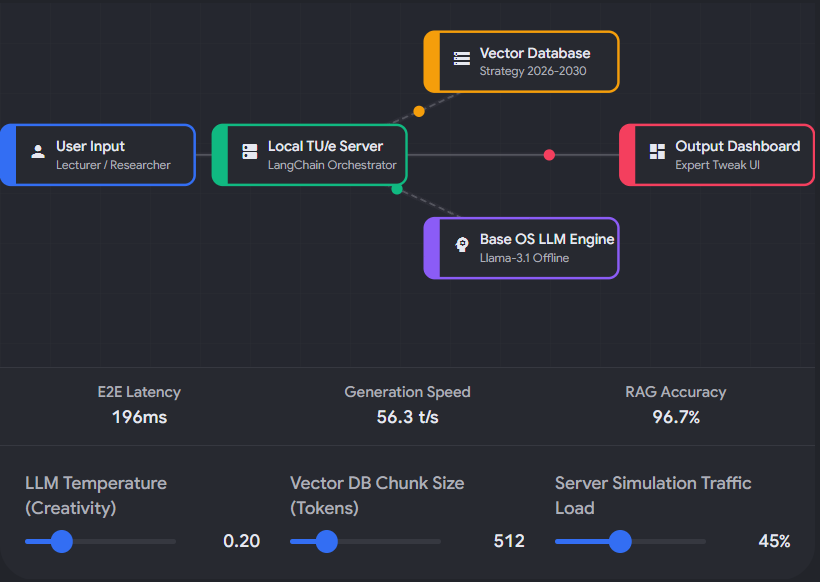
\includegraphics[width=0.9\textwidth]{assets/images/phase1/original-system-workflow.png}
\caption{Original architecture sketch. Displayed performance values are illustrative and have not been measured or validated.}
\label{fig:original-architecture}
\end{figure}

\begin{figure}[p]
\centering
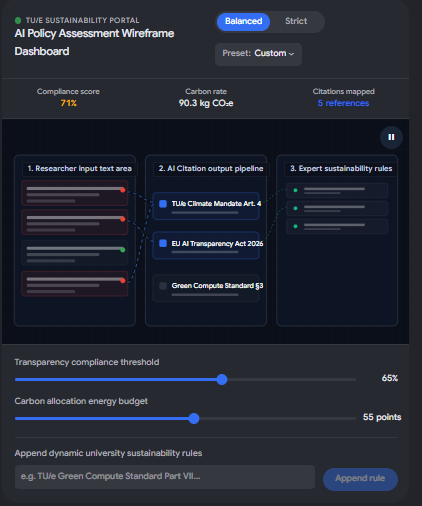
\includegraphics[height=0.68\textheight,keepaspectratio]{assets/images/phase1/original-dashboard.png}
\caption{Original dashboard sketch. Its scores and policy labels are unverified placeholders; the current proposal uses separate indicators without an overall score.}
\label{fig:original-dashboard}
\end{figure}

\FloatBarrier
\clearpage

% END embedded appendices/phase1-sketches.tex

\end{document}
